\section{\sysname{} Design}
\label{sec:design}

We first present an example to motivate our work, explain how we model
the distributed consistency semantics, and how applications can be
encoded into our \sysname{} framework.

\subsection{Motivating Example}
\label{subsec:eg}
Assume a movie streaming service built using a form of
microservice architecture where admins manage the serviced
contents and clients rent movies and leave reviews~\cite{deathstar}
(\needref{Fig}).
There are quite a few functionalities and components to build the
service, and it is nontrivial to meet all service requirements
and to guarantee that all requirements are fulfilled.

For example, a movie metadata database (DB) stores list of
available movies and each movie's information such as the
logline, director, and cast. This DB is accessed 1) when
the service admin adds/modifies movie information and
2) when clients reads the DB before renting a movie
or writing a review.

The developer of the system can choose an ACID database or linearizable
key-value store for the metadata DB but this may not scale well.
For utmost scalability and performance eventually consistent
key-value store can be used but users may observe anomalies.
Thus, to find a proper storage module, key constraints to satisfy for
each access
functionalities to minimize anomalous user experience needs to be defined: \eg
admins must always observe their own updates and clients must be able
to see what
they have previously seen. The collection of constraints should be satisfied
by the metadata DB of developer's choice, but if functionalities of the system
grow, the constraints can become more sophisticated and checking whether the
constrains are fully satisfied by a DB becomes more complicated.

While the metadata DB example above is presented in isolation from
what a single DB service must satisfy, cross DB constraints can exacerbate
the problem. For example, accessing the metadata DB would require
checking whether the user is an admin or a client with active movie subscription
status which may be maintained in a separate storage system, so
dependencies from the login service and the user DB must be fulfilled:
the user must be able to observe the user's valid up-to-date status
and then access the other services. Renting a movie or reading/writing a
review involves additional consistency constraints that cross storage services
for movies and reviews forming more complex dependencies that the system as a
whole must satisfy.

\sysname{} provides facilities to systematically encode the constraints
and check whether the constraints are all satisfied.

%\subsection{Modeling Consistency Semantics}
\subsection{Preliminaries}

\sysname{} provides pre-built pluggable \sysmodlong{} (\sysmods{})
that represent distributed storage services which can be checked whether
they are compatible with application constraints.
Each \sysmod{} models distributed consistency semantics introduced in
\cref{sec:background} and \cref{fig:semantics-tree}.
In the movie streaming service example, given all the constraints for the
metadata DB and the developer's \sysmod{} choice for the metadata DB,
\sysname{} can check if they are compatible. Also, given the constraints,
\sysname{} can search through existing \sysmods{} for compatible
consistency semantics.

\sysname{} follows the definitions provided by
Viotti et al.~\cite{viotti2016consistency} and others~\needcite{}
and uses predicate logic derived from the definitions to
model \sysmods{} and reason about consistency semantics with SMT solvers.
Consistency semantics are defined as logical formulas over axioms and
relations. Each model enforces safety properties, specifically ordering and
visibility constraints on operations within history and abstract
executions.

\para{Operations, Relations, and History.}
To model a consistency semantics for a \sysmod{}, we must first define an
operation, a tuple containing the following:
\itemparen{
\item \textit{proc:} the process that issued the operation, used for
session identification).
\item \textit{type:} the type of the operation such as read, write, or custom).
\item \textit{obj:} the object the operation is performed on.
\item \textit{ival:} operation input value.
\item \textit{oval:} operation output value.
\item \textit{stime:} invocation time of the operation.
\item \textit{rtime:} response time of the operation.
}
An operation
can be conceptualized as a request-response pair, where the request
is the operation itself and the response is the operation with the
response time set.

Consistency semantics are typically defined using universally
quantified formulas
(e.g., $\forall a, b: \dots$) applied to relations that are treated
as uninterpreted
functions of operations by the SMT solver
(e.g., $\text{vis}(a, b)$, $\text{so}(a, b)$).
Typically, they define pairwise constraints defined over operations in history.
A history is a set of operations that have been logically executed in the
\sysmod{}.
The functions representing the relations are used as base premises
for consistency
models and are used in axioms and invariants that the SMT solvers
interpret and check.

The relations defined for operations within a history include:
\itemparen{
\item returns-before: $\text{rb} \triangleq \{(a, b) : a, b \in H
\wedge a.\text{rtime} < b.\text{stime}\}$
\item same-session: $\text{ss} \triangleq \{(a, b) : a, b \in H \wedge
a.\text{proc} = b.\text{proc}\}$
\item session-order:
$\text{so} \triangleq \text{rb} \cap \text{ss}$
\item same-object: $\text{ob} \triangleq \{(a, b) : a, b \in H \wedge
a.\text{obj} = b.\text{obj}\}$
}

In our implementation, each history relation function (e.g.,
\texttt{History.Relation.returns\_before}) accepts an optional
\texttt{symbols} argument. This parameter allows framework users to
explicitly specify the symbolic operations, for example, \texttt{["a\_X",
"b\_X"]}), over which the relation's constraints should be quantified
for that specific instance \texttt{X}. This mechanism enables the application of
history-based constraints distinctly to operations belonging to
different modeled systems or components, contributing to the logical
isolation necessary for cross-system analysis.

\para{Abstract Execution (AE).}
An abstract execution instantiates and refines the history by
specifying which operations are visible to, or are arbitrated over
each other to model and check valid behaviors under a consistency semantics.
Abstract execution relations are non-deterministic
orderings used to capture more complex temporal constraints and
conflict resolution. The relationships include:
\itemparen{
\item \textit{Visibility (vis):} defines effects of write propagation
where the effect of
an operation is visible to the process invoking another operation.
\item \textit{Arbitration (ar):} an application specific, transitive and acyclic
relation that provides a total order on conflicting operations,
ensuring that observed executions follow a single coherent timeline.
\item \textit{Happens-before (hb):} used to capture probable causality,
and is previously defined in the literature as the transitive union
of session order and visibility: $hb \triangleq (\text{so} \cup
{\text{vis}})^{+}$
\
}
The formal definitions of these relationships can be found in prior
work~\cite{burckhardt2014principles,viotti2016consistency}
with the exception of visibility which we define in \cref{subsec:vis}.
These relations provide the foundation
for modeling sophisticated consistency guarantees that go beyond
simple temporal ordering, enabling the specification of complex
distributed system behaviors where operations may be reordered,
delayed, or selectively visible across different system components.
In other words, multiple AEs are possible for a
single history as observed event orderings can differ between nodes.
The AE encode the non-deterministic effects of asynchronous execution
environments and implementation-specific constraints.

\subsection{Base Consistency Semantics}
\label{subsec:semdef}
Based on the preliminaries, now we can discuss the formal definitions of
base consistency semantics, EC, MR, RYW, MW, WFR, PRAM, CC, and LIN, in
\cref{sec:background}.
The semantics are defined axiomatically using the relations between
pairwise operations (i.e., $a, b, \textrm{ and } c$ in a history $H$ of
operations, where $H_\text{wr}$ and $H_\text{rd}$ are histories of reads and
writes respectively.
While we adopt the definitions of MR, RYW, MW, WFR,
and PRAM of Viotti et al.~\cite{viotti2016consistency} (\cref{fig:semdef}),
we newly propose or augment EC, CC, and LIN for SMT encoding and
check their correctness with respect to other semantic definitions
using \sysname{}
(Section\needref{}).

\begin{figure}
\begin{eqnarray*}
\text{MW} & \triangleq & \forall a, b \in H_\text{wr}: a
\xrightarrow{\text{so}} b \Rightarrow a \xrightarrow{\text{ar}} b
\\
\text{RYW} & \triangleq & \forall a \in H_\text{wr}, \forall b \in
H_\text{rd}: a \xrightarrow{\text{so}} b \Rightarrow a
\xrightarrow{\text{vis}} b
\\
\text{MW} & \triangleq & \forall a, b \in H_\text{wr}: a
\xrightarrow{\text{so}} b \Rightarrow a \xrightarrow{\text{ar}} b
\\
\text{WFR} & \triangleq & \forall a, c \in H_\text{wr}, \forall b \in
H_\text{rd}: a \xrightarrow{\text{vis}} b \land b
\xrightarrow{\text{so}} c \Rightarrow a \xrightarrow{\text{ar}} c
\\
\text{PRAM} & \triangleq & \forall a, b \in H: a \xrightarrow{\text{so}}
b \Rightarrow a \xrightarrow{\text{vis}} b
\end{eqnarray*}
\caption{Formal definitions of monotonic reads (MR), read-your-writes
(RYW), monotonic writes (MW), write-follows-reads (WFR), and pipeline
RAM (PRAM) consistency.}\label{fig:semdef}
\end{figure}

\para{Eventual Consistency (EC).}
While EC definitions in other literatures
\cite{terry1994session, eventual, viotti2016consistency}
heavily focus on the liveness aspects using the concept of
eventual visibility of operations,
\sysname{} excludes liveness properties and concentrates on safety
properties:
%\itemparen{
%  \item
(1) non-circular causality, an acyclic projection of the happens-before
relation,
%\item
and (2) contextual return value consistency, a predicate on abstract
executions ensuring that the return value of any operation within
that execution belongs to the set of its valid return values
guided under the can-view relation which we define in \cref{subsec:vis}.
%}
\begin{align*}
&\text{EC}(\mathcal{F}) \triangleq \text{acyclic}(hb) \land \forall
op \in H: op.oval \in \mathcal{F}(op, ctx(A, op)) \\
% for all read op, the ival of operations thats in can-view relation with op
&\mathcal{F}_{\text{can-view}}(op, ctx(A, op)) = \{x.ival \in
H_\text{wr} : (op, x) \in \text{can-view}\}
\end{align*}

\para{Causal Consistency (CC).}
Our CC formulation combines concepts from Viotti et
al.~\cite{viotti2016consistency} and causal
memory~\cite{baldoni2002an}. The \textit{writes-into (wi)}
relation~\cite{baldoni2002an} connects write operations directly with the
reads that retrieve their values. This guarantees that when
a read operation observes a specific write, all following writes
within the same session honor that causal sequence. The formalization
coordinates session order, arbitration, visibility, and writes-into to
preserve consistent causal histories.

Operations belong to the \texttt{wi} set when: a write $a$
writes into a read $b$ if and only if $b$ retrieves the value initially written
by $a$, and $a$ and $b$ access the same object (or identical memory region).
Each $b$ can have at most one corresponding $a$, maintaining acyclicity.
When one operation succeeds another in session order, their
relationship within the abstract execution faces additional constraints.
Particularly, if $(a, b) \in \text{so}$, then $a$ must write-into $b$ when
$b$ represents a read operation, and $a$ must be visible and
arbitrated prior to $b$. Consequently, session order establishes a causal
sequence that manifests in the relations wi, vis, and ar.
%$$
\begin{eqnarray*}
\text{CC} \triangleq \text{WFR} \land \forall a, b \in H: (a, b) \in
\text{so} \Rightarrow (a, b) \in \text{wi} \cap \text{vis} \cap \text{ar}
\end{eqnarray*}
%$$
These constraints collectively establish a causal memory model where
session order, observed values, and write sequences maintain alignment, ensuring
causally dependent writes manifest in proper order from any
observer's viewpoint.

\para{Liniearizability (LIN).} In our encoding of LIN,
we introduce a modified single global order constraint to unify visibility and
arbitration for all write operations regardless of operations in
session-based semantics or not, and enforce real-time ordering to
ensure that the observed histories comply with returns-before relations:
i.e., linearization as operations comes in instead of lazily ordering
events when
reads occur \cite{zhang2018building}.
\begin{eqnarray*}
\text{LIN} & \triangleq & (\forall a, b \in H: [a
\xrightarrow{\text{vis}} b \implies a \xrightarrow{\text{ar}} b] \land  \\
& & [a \xrightarrow{\text{ar}} b \land a.rtime < \infty \implies
a \xrightarrow{\text{vis}} b]) \\
& & \land rb \subseteq ar \\
& & \land \forall x \in H: x.oval \in \{y.ival \in H_\text{wr} : (x,
y) \in \text{can-view}\}
\end{eqnarray*}

\subsection{Formal Definitions of ``Visibility''}
\label{subsec:vis}
One of our key contributions is formally defining visibility.
Although visibility is used as part of defining almost all semantics in
\cref{subsec:semdef} and \cref{fig:semdef}, its definitions in
existing literatures are informal and ambiguous regarding exact
behavior under concurrent
settings~\cite{viotti2016consistency,viotti2016towards,zhang2018building,ferreira2023antipode}.
As with many seemingly simple informal definitions surrounding
concurrent and distributed environments, formally defining visibility
for use in \sysname{}-like tools is non-trivial.
We restructure visibility as a binary relation
and perform explicit case analysis on all possible combinations of
read and write operations that can be \textit{visible} to each other.

\begin{figure}[tb]
\centering
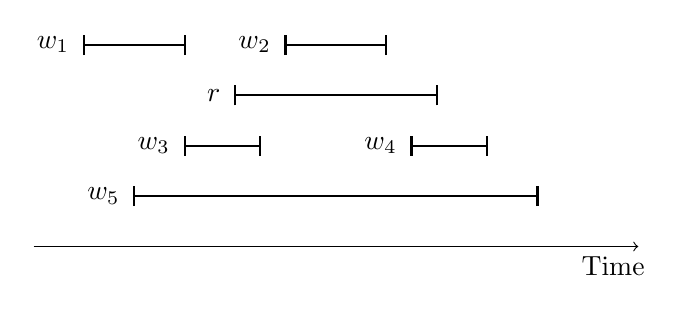
\begin{tikzpicture}[scale=0.64]
% time
\draw[->] (0,1) -- (12,1);
\node[below] at (11.5,1) {Time};

\draw[thick] (1,5) -- (3,5);
\draw[thick] (1,4.8) -- (1,5.2); % left terminating bar
\draw[thick] (3,4.8) -- (3,5.2); % right terminating bar
\node[left] at (0.9,5) {$w_1$};

\draw[thick] (5,5) -- (7,5);
\draw[thick] (5,4.8) -- (5,5.2); % left terminating bar
\draw[thick] (7,4.8) -- (7,5.2); % right terminating bar
\node[left] at (4.9,5) {$w_2$};

% middle
\draw[thick] (4,4) -- (8,4);
\draw[thick] (4,3.8) -- (4,4.2);  % left terminating bar
\draw[thick] (8,3.8) -- (8,4.2);  % right terminating bar
\node[left] at (3.9,4) {$r$};

\draw[thick] (3,3) -- (4.5,3);
\draw[thick] (3,2.8) -- (3,3.2);   % left terminating bar
\draw[thick] (4.5,2.8) -- (4.5,3.2); % right terminating bar
\node[left] at (2.9,3) {$w_3$};

\draw[thick] (7.5,3) -- (9,3);
\draw[thick] (7.5,2.8) -- (7.5,3.2); % left terminating bar
\draw[thick] (9,2.8) -- (9,3.2);   % right terminating bar
\node[left] at (7.4,3) {$w_4$};

\draw[thick] (2,2) -- (10,2);
\draw[thick] (2,1.8) -- (2,2.2);   % left terminating bar
\draw[thick] (10,1.8) -- (10,2.2); % right terminating bar
\node[left] at (1.9,2) {$w_5$};
\end{tikzpicture}
\caption{The can-view relation captures the
possible visibility between read and write operations. The
read-write pairs $r$ and $w_1$, $w_2$, $w_3$, $w_4$, $w_5$ are
defined based on their start and return times, where the read
operation can view the effect of the write operations if they fall
into one of the cases defined in the can-view relation.}
\label{fig:can-view}
\end{figure}

We introduce the notion of \textit{can-view} and \textit{viewed} to capture the
deterministic and non-deterministic behavior of operations,
and what it means for one operation to be able to \textit{observe}
the effects of another operation. To achieve visibility, two
operations must first fall in one of
the categories in \textit{can-view}: either (1) the write happened
before the read
in absolute time (note that whether the read/write happened on the
same process does not matter, as synchronization
is not required to establish probable effect causality)
or (2) the read and write happened concurrently such that the read might
observe the write's effect (\cref{fig:can-view}).
%
Formally, this can-view relation, $a \xrightarrow{\text{can-view}} b$,
is defined over the pairwise start or return time of read $a$ and
write $b$ operations:
%When two operations
%$a$ and $b$ are defined to be in can-view relation
%($a \xrightarrow{\text{can-view}} b$), either $a$ returned before
% $b$, such that $b$'s write effect can be visible to $a$, or $a$ and
% $b$ happened concurrently such that
%$b$'s write effect might be visible to $a$.
\begin{eqnarray*}
\text{can-view} & \triangleq & \{(a, b) : a \in H_\text{rd}, b \in
H_\text{wr} \land a.\text{obj} = b.\text{obj} \\
& & \land ((a.\text{stime} > b.\text{rtime}) \\
& & \quad\lor (a.\text{stime} \leq b.\text{stime} \land
a.\text{stime} \leq b.\text{rtime} \land \\
& & \quad\quad\ \ a.\text{rtime} \geq b.\text{stime} \land
a.\text{rtime} \geq b.\text{rtime}) \\
& & \quad\lor (a.\text{stime} \geq b.\text{stime} \land
a.\text{stime} \leq b.\text{rtime} \land \\
& & \quad\quad\ \ a.\text{rtime} \geq b.\text{stime} \land
a.\text{rtime} \geq b.\text{rtime}) \\
& & \quad\lor (a.\text{stime} \leq b.\text{stime} \land
a.\text{stime} \leq b.\text{rtime} \land \\
& & \quad\quad\ \ a.\text{rtime} \geq b.\text{stime} \land
a.\text{rtime} \leq b.\text{rtime}) \\
& & \quad\lor (a.\text{stime} \geq b.\text{stime} \land
a.\text{stime} \leq b.\text{rtime} \land \\
& & \quad\quad\ \ a.\text{rtime} \geq b.\text{stime} \land
a.\text{rtime} \leq b.\text{rtime}
)
)\}.
\end{eqnarray*}

While can-view captures the possible visibility between read and write, the
result dependency between them is captured by the \textit{viewed} relation:
\begin{eqnarray*}
\text{viewed} & \triangleq & \{(a, b) : a \in H_\text{rd}, b \in H_\text{wr} \\
& & \land (a, b) \in \text{can-view} \\
& & \land (
(a.\text{oval} = b.\text{ival})\lor \\
& &
\text{ }(\exists x \in H_\text{wr} : (x, b) \in
\text{can-view} \land a.\text{oval} = x.\text{ival})
)
\}
\end{eqnarray*}
The viewed relation is defined as a non-deterministic
pairwise partial ordering
between a read and a write that builds upon can-view. Aside from timestamps
falling into one of the can-view cases, we
assign additional value-related constraints to operations: either the value
written by the write operation must match the output
of the read, or, in case of another write operation that happened after or
concurrently to the aforementioned write, the viewed relation enforces the
output of the read to be from one of the writes (but only one can be chosen).
In the visibility definition, the transitivity of the viewed relation
is implicitly
enforced.

Using Figure \ref{fig:can-view}'s operations $r$ and $w_1$ as an example,
since $r$ and $w_1$ are in the can-view relation, if $w_1$'s written
value matches $r$'s output, then $r$ is in the viewed relation with $w_1$.
Consider another operation $w_5$ in the same figure that happened
concurrently with $w_1$. If $w_5$'s written value differs
from $w_1$, but $r$ and $w_5$ are in the can-view relation and $r$ and
$w_5$ have value equivalence, then $r$ and $w_1$ are still in the viewed
relation (write $w_1$ still affects $r$).
However, in this scenario, the constraint in effect for the viewed
relation is the existence of $w_5$ and the value equivalence of $r$ and $w_5$.

% actual vis
Finally, the \textit{visibility (vis)} definition establishes a
deterministic pairwise
relationship between any two operations in the history
rather than being limited to read-write pairs.
It also adds the transitivity (propagation) and acyclicity
(cannot go back in time) to the viewed relation.
These were not enforced in our original viewed definition to preserve
non-determinism in ordering concurrent operations and to include all pairs of
operations that can be viewed by each other.
When constraint $a \xrightarrow{\text{vis}} b$ is assigned to a pair
of operations,
the following cases are considered:
\begin{align*}
\text{vis} & \triangleq \{(a, b) : \\
& (a \in H_\text{rd}, b \in H_\text{rd} : \exists x \in
H_\text{wr}: (x, a) \in \text{vis} \Rightarrow (x, b) \in \text{vis}) \\
& \lor
(a \in H_\text{rd}, b \in H_\text{wr} : \exists x \in
H_\text{wr}: (x, a) \in \text{vis} \Rightarrow (x, b) \in \text{vis}) \\
& \lor
(a \in H_\text{wr}, b \in H_\text{rd} : \text{viewed} \subseteq
\text{ar}) \\
& \lor
(a \in H_\text{wr}, b \in H_\text{wr} : (a, b) \in \text{ar})\}.
\end{align*}
%\end{eqnarray*}
Note that the read-read and read-write cases are recursively
defined,
%
%where $a$ and $b$ are in $\text{vis}_\text{rd-rd}$ or
%$\text{vis}_\text{rd-wr}$, if and only if there exists a
%write $x$ that is
%visible to $a$, and $x$ is in $\text{vis}_\text{wr-rd}$ or
%$\text{vis}_\text{wr-wr}$ with $b$.
%
We call this the
write propagation rule. Conceptually, this means that if a read $r$
and another operation (either read or write) $x$ are in the visibility relation,
the closest write operation $w$ that is visible to read $r$ must
be propagated to $x$. Whether this visibility relation can be satisfied
depends solely on the existence of read $r$'s previous and
immediately adjacent write operation $w$, and whether
that $w$ can satisfy the write-read or write-write pairwise
constraints of visibility.

Write-read case is straignforward:
%we term this rule definitive
%visibility. Definitive visibility is defined as follows:
if a write $w$ is visible to a read $r$, then $r$
must have viewed $w$ and an arbitration relation must exist between $w$ and $r$
to ensure the non-deterministic viewed relation has a
linearization point, i.e., to cut off one of the possible paths in
the viewed relation.
Then what does it mean for writes to be visible to writes? This translates to
write arbitration: whether two writes are visible to each other depends on the
existence of an arbitration relation between them.
Writes unordered by visibility is considered invisible to each
other~\cite{viotti2016consistency}
and the arbitration resolves conflicts in concurrent and invisible operations.

With the complete visibility definition we encode the aformentioned semantics
into \sysname{} which are then used to reason about the compatibility
between applications and semantics/systems.

%Other relations under Abstract Execution includes arbitration, and
%happens-before.
%Arbitration is an application specific, transitive and acyclic
%relation that provides a total order on conflicting operations,
%ensuring that observed executions follow a single coherent timeline. In
%our implementation, arbitration is assigned strong timestamp total ordering.
%Realistically, arbitration can be achieved with monolithic
%sequencers, deterministic
%conflict resolution rules, distributed timestamping \cite{lamport1978time},
%or consensus protocols
%\cite{birman1991lightweight,hadzilacos1994modular,lamport2001paxos}.
%Happens-before is used to capture probable causality,
%and is previously defined in the literature as the transitive union
%of session order and visibility:
%$hb \triangleq (\text{so} \cup {\text{vis}})^{+}$
%\cite{burckhardt2014principles,viotti2016consistency}.

%Operations do not contain the node that issued or
%handled the operation; they are defined as generic entities that can
%be issued by any node and handled by any node. To add constraints on
%the nodes that can issue or handle an operation, the \sysname{} user
%must define nodes and edges.

%By assigning unique symbols to operations (and potentially
% relations) associated
%with different components (e.g., $a_X$, $b_X$, $\text{vis}_X$ for
%System X; $a_Y$, $b_Y$, $\text{vis}_Y$ for System Y), we maintain
%the necessary logical isolation. This ensures that the axioms and
%constraints of a specific consistency model only apply to the
%operations within that specific system's scope. This symbolic
%separation is fundamental for enabling the analysis of
%cross-system interactions, where specific ``glue''
%constraints can then be added explicitly to relate operations across
%these distinct symbolic domains, as demonstrated in our cross-causal
%consistency modeling.
